\chapter{Results}
\label{chap:results}


This chapter first explores the behavior of Sum and Product Coupling.
Then it compares to PAIRpred and the other variants of graph convolution.
Some convolution filters are then visualized, along with network output for one trained network.
Finally, it summarizes the effect of protein size on network training time.


\section{Sum and Product Coupling Performance}

\begin{table}
	\begin{center}
		\begin{tabular}{lccccc}
			\toprule
			\multirow{2}{*}{Method} &
			Receptive Field & \multicolumn{4}{c}{Layers Before Merge} \\
			& Size & 1 & {2} & {3} & {4} \\
			\midrule
			No Convolution & N/A & \textbf{0.815} & 0.812 & 0.800 & 0.811  \\\cline{1-6}
			\multirow{2}{*}{Sum Coupling} & 11 & 0.868 & 0.889 & 0.882 & 0.884 \\
			& 21 & 0.875 & \textbf{0.903} & 0.880 & 0.890 \\\cline{1-6}
			\multirow{2}{*}{Product Coupling} & 11 & 0.856 & 0.869 & 0.885 & 0.868 \\
			& 21 & 0.863 & 0.876 & 0.896 & \textbf{0.899} \\
			\bottomrule
		\end{tabular}
		\caption{Median area under the receiver operating characteristic curve (AUC) across all complexes in the test set for two variants of graph convolution, Sum Coupling and Product Coupling, as well as No Convolution. Results are shown for two different sizes of receptive field, 11 and 21, for different numbers of convolutional layers before the pairwise merge operation. Bold faced values indicate best performance for each method.
		\label{tab:med_auc}}
	\end{center}
\end{table}

Table \ref{tab:med_auc} shows the results of experiments involving Sum Coupling and Product Coupling, as well as No Convolution.
Comparing Sum and Product Coupling to No Convolution reveals that convolution is beneficial.
In other words, incorporating information from neighboring residues helps indicate whether a residue is part of an interface, which is consistent with the biological properties of interfaces.
It's also clear that a receptive field of size 21 is generally better than 11.
Interestingly, this value is near the median number of interface residues for a single protein, which is 27.
When using convolution, performance improves with network depth up to a point, then either decreases or remains relatively constant.
In Sum Coupling, this maximum occurs in the second layer, whereas in Product Coupling, this maximum occurs in the fourth layer.
Though not shown in the table, Product Coupling indeed fails to improve when using 5 or 6 layers.
In contrast, networks without convolution are best with only one pre-merge layer.
This suggests that depth alone does not improve performance, but when convolution is performed, a useful hierarchical representation is learned.
Other applications of deep learning have seen this same trend of increasing and decreasing performance.
The commonly given explanations for such behavior include insufficient training data, a vanishing gradient, and a difficulty with optimization~\cite{he2015}.
Overall, both Sum and Product Coupling achieved similar performance in AUC.

\begin{table}
	\begin{center}
		\begin{tabular}{lccccc}
			\toprule
			\multirow{2}{*}{Method} &
			Receptive Field & \multicolumn{4}{c}{Layers Before Merge} \\
			& Size & 1 & {2} & {3} & {4} \\
			\midrule
			No Convolution & N/A & \textbf{48} & 55 & 53 & 66 \\\cline{1-6}
			\multirow{2}{*}{Sum Coupling} & 11 & 32 & 28 & 70 & 86 \\
			& 21 & \textbf{26} & 37 & 56 & 63 \\\cline{1-6}
			\multirow{2}{*}{Product Coupling} & 11 & 30 & 46 & 26 & 51 \\
			& 21 & 26 & \textbf{25} & 36 & 37 \\
			\bottomrule
		\end{tabular}
		\caption{Median rank of the first positive prediction (RFPP) across all complexes in the test set for two variants of graph convolution, Sum Coupling and Product Coupling, as well as No Convolution. Results are shown for two different sizes of receptive field, 11 and 21, for different numbers of convolutional layers before the pairwise merge operation. Bold faced values indicate best performance for each method (lower is better).}
		\label{tab:med_rfpp}
	\end{center}
\end{table}

Table \ref{tab:med_rfpp} parallels Table \ref{tab:med_auc} but shows RFPP instead of AUC.
As before, Sum and Product Coupling perform similarly to each other, and both outperform No Convolution.
In this case, however, the best performance for Sum and Product Coupling is seen for fewer layers than AUC.
This difference is not surprising, considering the cross-entropy loss function leads to optimization of performance on \emph{all} pairs, not just the top scoring ones.
In other words, RFPP is not being explicitly optimized in this problem, whereas AUC is more closely related to the quantity being optimized.

\begin{figure}
	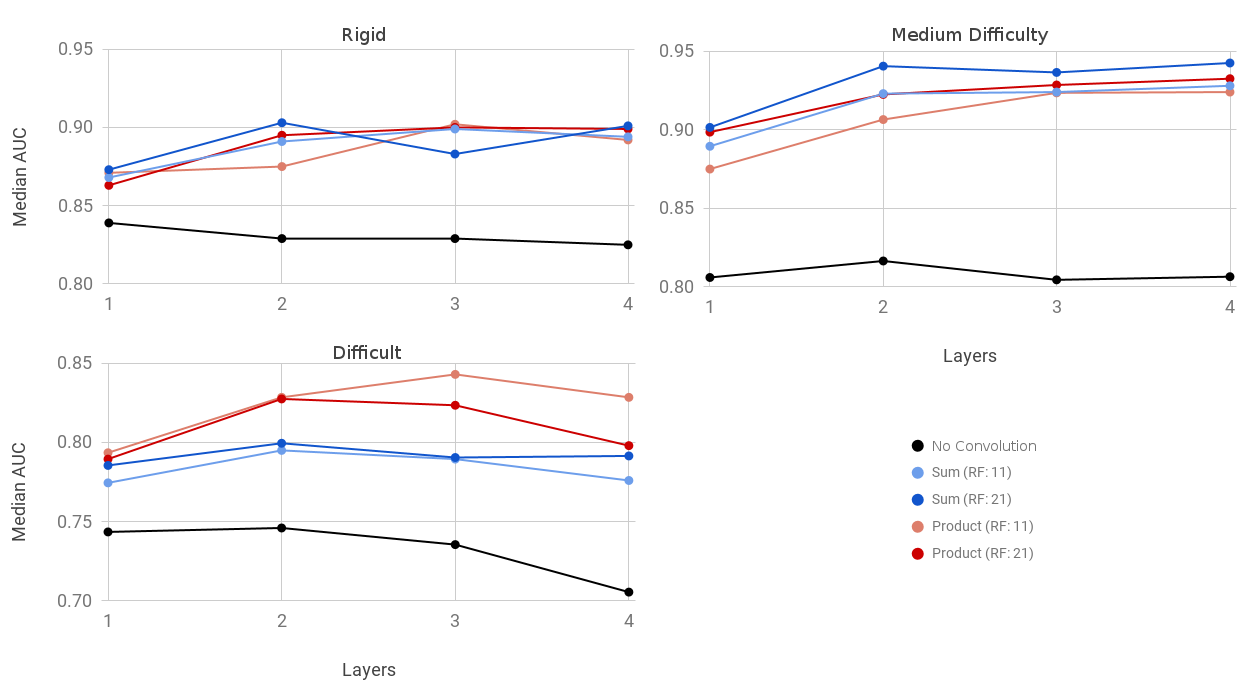
\includegraphics[width=\textwidth]{med_auc.png}
	\caption{Median area under the receiver operating characteristic curve (AUC) across all complexes in the test set, separated by complex class. Sum and Product Coupling are shown for two receptive field sizes each (11 and 21), as well as No Convolution, for 1-4 pre-merge layers. Product Coupling performs better for difficult complexes, but worse overall because ther are far more rigid and medium difficulty complexes.
		\label{fig:med_auc}}
\end{figure}

To understand the behavior of each method in more detail, we can separate performance by the difficulty class of the test proteins.
Figure \ref{fig:med_auc} shows performance for rigid, medium difficulty, and difficult classes, with 33, 16, and 6 complexes respectively.
Here it appears that Sum and Product Coupling are closely matched for rigid and medium difficulty.
A slight difference is seen for the difficult complexes, where Product Coupling appears to be performing better for two and three layers, but with so few complexes it's unclear if this is a true trend.

\begin{figure}
	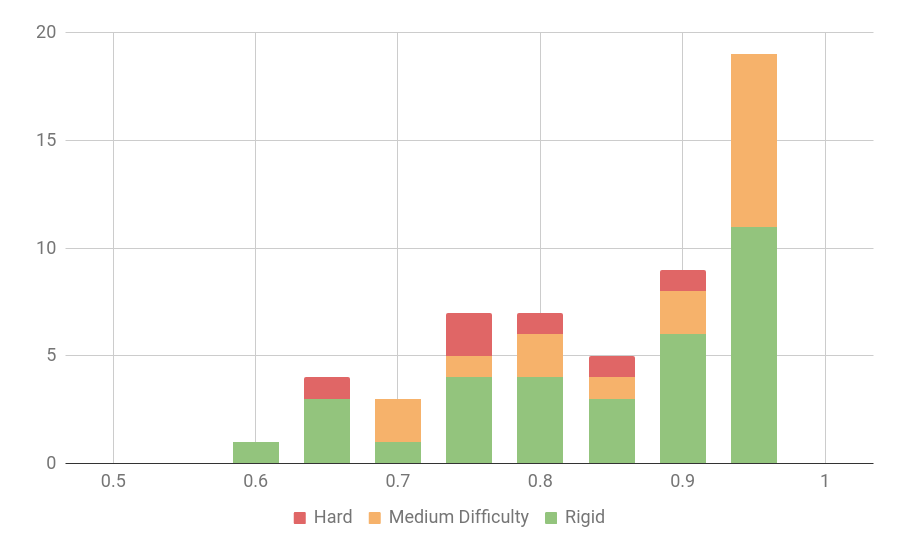
\includegraphics[width=0.8\textwidth]{sum_20_2_histo1.png}
	\caption{Histogram of area under the receiver operating characteristic curve (AUC) for complexes in the test set, colored by difficulty class. Scores are from Sum Coupling with two layers and receptive field size 21, which had the highest median AUC of all methods.}
	\label{fig:histo1}
\end{figure}

For another picture of performance across difficulty classes, we can examine a histogram of AUCs, as shown in Figure \ref{fig:histo1}.
These AUCs are heavily skewed, justifying the choice of median as a summary measure.
Surprisingly, there is no clear divide between rigid, medium difficulty, and difficult classes.
In fact, the worst AUC is a rigid complex, and one difficult complex achieves AUC above 0.9.
It appears that the distinguishing characteristic between classes is the number of complexes that achieve above 0.95 AUC.
These "trivial" complexes are most frequent in the rigid class, less so in the medium difficulty class, and absent for the difficult class.
This suggests that the networks are effectively coping with some complexes that under conformational change.

\begin{figure}
	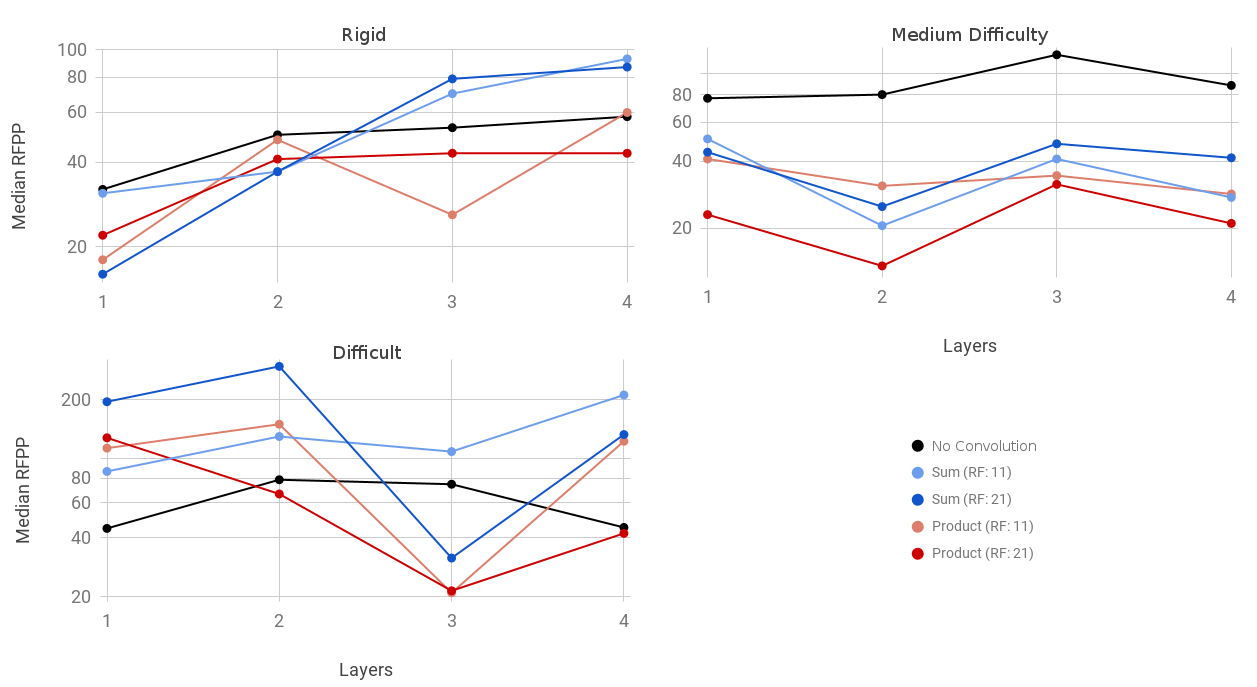
\includegraphics[width=\textwidth]{med_rfpp.png}
	\caption{Median rank of the first positive prediction (RFPP) across all complexes in the test set, separated by difficulty class. Vertical axes are log scaled. Sum and Product Coupling are shown for two receptive field sizes each (11 and 21), as well as No Convolution, for 1-4 pre-merge layers. Lower RFPP is better. Best performance on rigid complexes is achieved with just one layer for all networks. As difficulty increases, so does the number of layers needed to achieve best results.
		\label{fig:med_rfpp}}
\end{figure}

RFPP can also be separated by difficulty class.
From figure \ref{fig:med_rfpp} we can observe some heterogeneus behavior across methods, but there are some trends worth noting.
For each class, there appears to be a favored number of layers where a dip (improvement) in RFPP is observed. 
This optimal depth appears to increase with difficulty class, suggesting that harder complexes require more layers to achieve best performance.
Therefore an ensemble approach with varying depths may perform well on complexes of any difficulty. 



\section{Comparison to Other Methods}


\begin{table}
	\begin{center}
		\begin{tabular}{l c c c c c }
			\toprule
			
			
			\multirow{2}{*}{Method} & \multirow{2}{*}{Variant} &  \multicolumn{4}{c}{Layers} \\
			& & 1 & 2 & 3 & 4 \\
			
			\midrule
			No Convolution & N/A & \textbf{0.815} & 0.812 & 0.800 & 0.811 \\
			\midrule
			\multirow{2}{*}{Sum Coupling} & $\text{RF}=11$ & 0.868 & 0.889 & 0.882 & 0.884 \\
			& $\text{RF}=21$ & 0.875 & \textbf{0.903} & 0.880 & 0.890 \\
			\midrule
			\multirow{2}{*}{Product Coupling} & $\text{RF}=11$ & 0.856 & 0.869 & 0.885 & 0.868 \\
			& $\text{RF}=21$ & 0.863 & 0.876 & 0.896 & \textbf{0.899} \\
			\midrule
			PAIRpred~\cite{minhas2014}   & N/A  & (\textbf{0.863})* & - & - & - \\
			
			\midrule
			\multirow{2}{*}{PATCHY-SAN~\cite{niepert2016}}  & $\text{RF}=11$ & 0.862 & 0.867 & 0.883 & 0.891 \\
			& $\text{RF}=21$ & 0.850 & 0.875 & \textbf{0.897} & 0.886 \\
			\midrule
			\multirow{2}{*}{Fingerprint~\cite{duvenaud2015}}  & $\text{RF}=11$ & 0.857 & 0.850 & 0.863 & 0.833 \\
			& $\text{RF}=21$ & 0.861 & 0.867 & 0.881 & \textbf{0.891} \\
			\midrule
			
			\multirow{6}{*}{R-GCN~\cite{schlichtkrull2017}} & No basis fns, $\text{RF}=11$ & 0.862 & 0.871 & 0.886 & 0.893 \\
			& No basis fns, $\text{RF}=21$ & 0.876 & \textbf{0.901} & 0.892 & 0.897 \\
			& 2 basis fns, $\text{RF}=11$ & 0.851 & 0.872 & 0.779 & -	   \\
			& 2 basis fns, $\text{RF}=21$ & 0.873 & 0.804 & 0.539 & -     \\
			& 5 basis fns, $\text{RF}=11$ & 0.870 & 0.747 & 0.748 & -	   \\
			& 5 basis fns, $\text{RF}=21$ & 0.867 & 0.900 & 0.709 & -     \\
			\midrule
			\multirow{2}{*}{DTNN~\cite{schutt2017}}& $\text{RF}=11$ & 0.853 & 0.872 & 0.878 & 0.861 \\
			& $\text{RF}=21$ & 0.862 & 0.880 & 0.873 & \textbf{0.885} \\
			\midrule
			\multirow{4}{*}{DCNN~\cite{atwood2016}} & 2 hops, $\sigma=2$\AA{} & 0.782 & - & - & - \\
			& 2 hops, $\sigma=4$\AA{} & 0.801 & - & - & - \\
			& 5 hops, $\sigma=2$\AA{} & \textbf{0.838} & - & - & - \\ 
			& 5 hops, $\sigma=4$\AA{} & 0.819 & - & - & - \\ 
			
			\bottomrule
			
		\end{tabular}
		\caption{Comparison of proposed convolutions with existing classification methods. Bold values indicate best performance for each method. For reference, retraining Sum Coupling ten times with a different random seed yields a standard deviation of 0.006, and other methods are believed to behave similarly. *PAIRpred is an SVM-based approach, so the result is not really associated with a layer number.}
		\label{tab:results_compare}
	\end{center}
	%\end{minipage}
\end{table}

Table \ref{tab:results_compare} compares the median AUC of the various existing methods discussed.
PAIRpred, the state of the art pairwise interface predictor, establishes the baseline.
Interestingly, most of the graph convolution based methods exceed this.
DCNN is the exception, showing worse performance than PAIRpred.
This is perhaps unsurprising, since it differs considerably from the other convolution methods, which are very similar to one another.

The order imposing PATCHY-SAN performs quite well, suggesting that the chosen ordering of neighbors by proximity to the central vertex was a good one.
Its best AUC of 0.897 is within one standard deviation (0.006) of the best overall performance, which was 0.903 from Sum Coupling.
Therefore it is difficult to say whether order-free or ordered methods perform better for this problem.
Only one ordered method was examined, leaving the possibility that others may do better.
Because of the unique weights used for each neighbor, ordered methods have significantly more parameters than order-free methods, making them more susceptible to overfitting, though that is not observed in these results.
This method also uses information from all edges in the receptive field, whereas the other methods are only concerned with edges connecting neighbors to the central vertex.

R-GCN did the best without basis matricess.
The original intent for basis matricess was to allow for weight sharing across several relation types.
This is less relevant for these protein graphs since only a single neighborhood is being considered per central vertex, so in a sense there is only one relation type.
When using basis matricess, larger networks (starting at three layers) drop significantly in performance compared to other methods.
At four layers, networks consistently classified all residue pairs with the same score, suggesting all filters had become zero valued (note that AUC cannot be calculated with all scores are identical).
Note that AUC cannot be calculated when all scores are identical.
This is possible when using ReLU nonlinearities, since the output and gradient vanishes for signals less than zero.
It's possible that a different initialization scheme or a different nonlinearity would remedy this problem.
Regardless, the use of basis matricess in this context is somewhat unjustified because these graphs lack the numerous relation types that prompted use of basis matricess in the first place~\cite{schlichtkrull2017}.
Nevertheless, the two layer, five basis matrices version performed similarly to the best results observed.
But testing with 8 basis matrices did not show improvement.
Without basis matricess, R-GCN is equivalent to Sum Coupling if edge information is excluded.
The fact that R-GCN without basis matricess performs similarly to Sum Coupling suggests that the added edge information in Sum Coupling is not very useful.

Fingerprint is arguably the simplest form of graph convolution since it uses the same weight matrix for both central and neighbor vertices.
Its best performance is only 0.01 below that of R-GCN, but it requires twice as many layers.
The number of layers to five or six exhibits no substantive improvement. 

Whereas PATCHY-SAN, Fingerprint, and R-GCN are most similar to Sum Coupling, DTNN allows for a multiplicative coupling between neighbors and edges, similar to Product Coupling.
Like Product Coupling, best performance is achieved at a greater depth than the other methods, but does not continue to improve for five or six layers. 
This method is notably worse than the three just mentioned.
One potentially limiting aspect of this method is that the number of channels is necessarily unchanged.
This may explain why this method performs worse than Product Coupling.


For DCNN, five hops performs better than two hops, presumably for the same reason that a larger receptive field is better in the other convolution methods: information is able to propagate further across the graph.
The Gaussian standard deviation determines the range of diffusion, where smaller values limit diffusion to a localized neighborhood for each hop, and larger values allow diffusion across longer distances.
In the two hop DCNN, the larger standard deviation allows more diffusion to occur across the graph, compensating for the limited number of hops.
This explains the overall better performance for $\sigma=4\AA{}$.
In contrast, the five hop DCNN performed better for $\sigma=2\AA{}$, suggesting that the larger number of hops allows sufficient information propagation, eliminating the need for diffusion across greater distances for each hop.





\section{Filter Visualization}

It is often difficult to understand the behavior of a model by simply looking at the overall performance. 
For convolutional neural networks on images, intuition can be gained through a variety of methods, including visualizing filters directly, tracking a filter's activation as different regions of the image are occluded, and identifying which images maximally activate each filter. 
To understand the filters being learned in this pairwise neural network architecture, network scores and filter activations were mapped to a protein complex heatmap.
Figure \ref{fig:filter_vis} presents color maps on the complex 3HI6 which depict the true interface, maximum predicted scores for each residue, and the activation of two filters from last convolutional layer, for the best performing method (Sum Coupling with two layers and receptive field size of 21).
Scores are partner specific, so they are shown for a single residue after taking the maximum over all potential partners.
This partner independent visualization matches well with the true interface.
In contrast, convolutional filters occur at the residue level and can be visualized directly. 
The two filters shown illustrate learned features which are useful for interface prediction.
Specifically, one activates only for buried residues (indicating an \emph{unlikeliness} to participate in an interface), and the other activates only for residues near the true interface.

\begin{figure}
	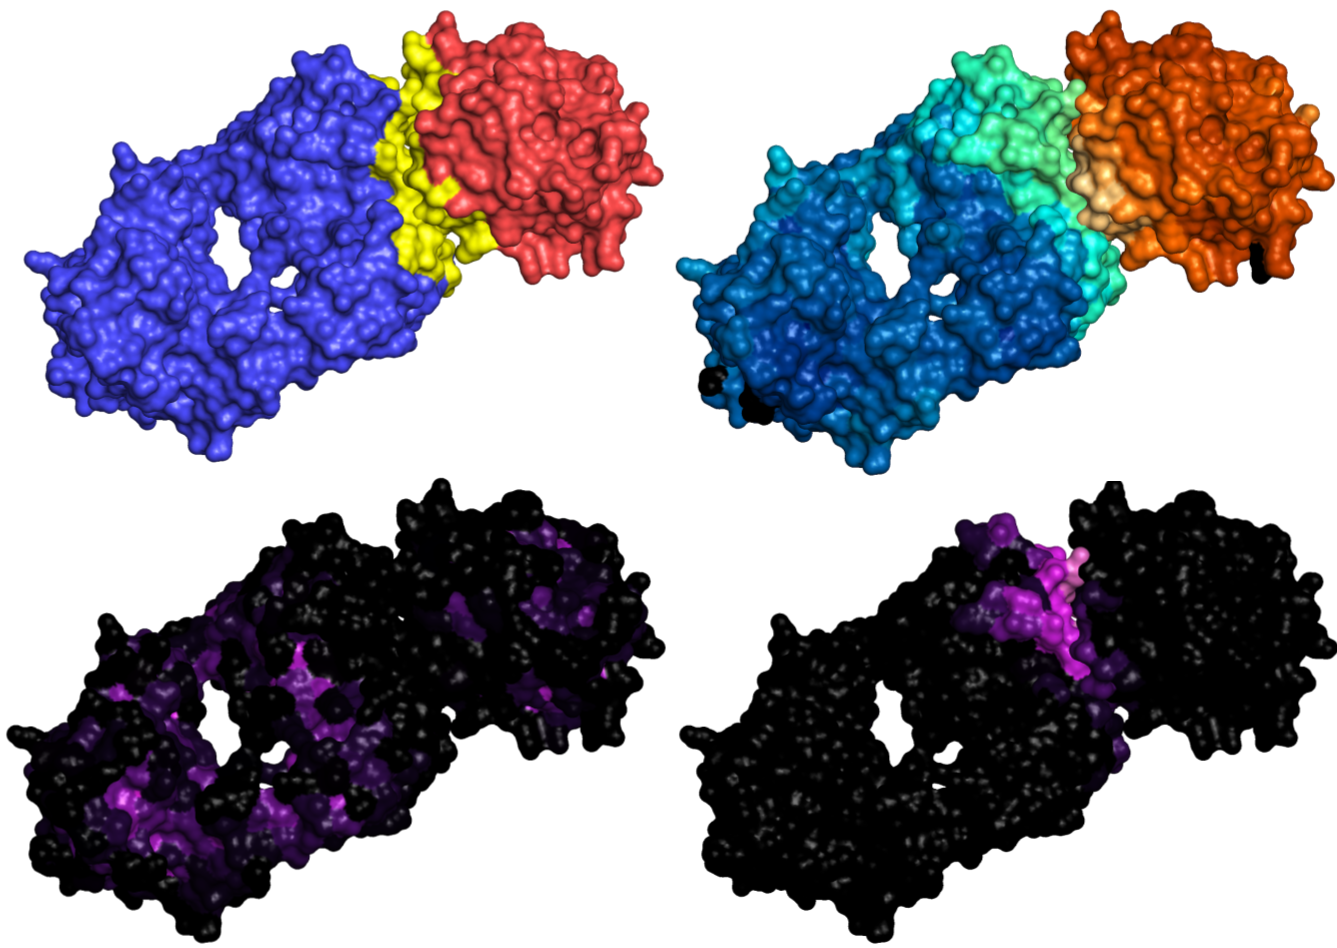
\includegraphics[width=0.6\textwidth]{3HI6_collage.png}
	\caption{PyMOL~\cite{schrodinger2015} visualizations of the best performing test complex (3HI6). Upper left: Ligand (red) and receptor (blue), along with the true interface (yellow). Upper right: Visualization of predicted scores, where brighter colors (cyan and orange) are higher scores and darker colors (blue and red) are lower scores. Since scores are for pairs of residues, we take the max score over all partners in the opposing protein. Bottom row: Activations of two filters in the second convolutional layer, where brighter colors indicate greater activation and black indicates activation of zero. Lower left: Filter which provides higher activations for buried residues, a useful screening criterion for interface detection. Lower right: Filter which gives high activations for residues near the interface of this complex.
		\label{fig:filter_vis}}
\end{figure}


\section{Training Time}

Figure \ref{fig:train_times} shows a log-log plot of training time as a function of the number of residue pairs in a given complex.
The relationship is roughly linear in this space, indicating a power-law relationship.
Fitting lines to the data shows that the power is slightly greater than 1.0 in all cases, showing that training time increases near linearly in the number of pairs as expected.
This is due to the pairwise nature of the problem.
For problems on a single graph, the training time would likely scale near linearly in the number of vertices.
Deeper networks take longer to train, and summing over neighbors (as in Product Coupling), takes longer than just using the central vertex (as in No Convolution).
These trends are as expected. 


\begin{figure}
	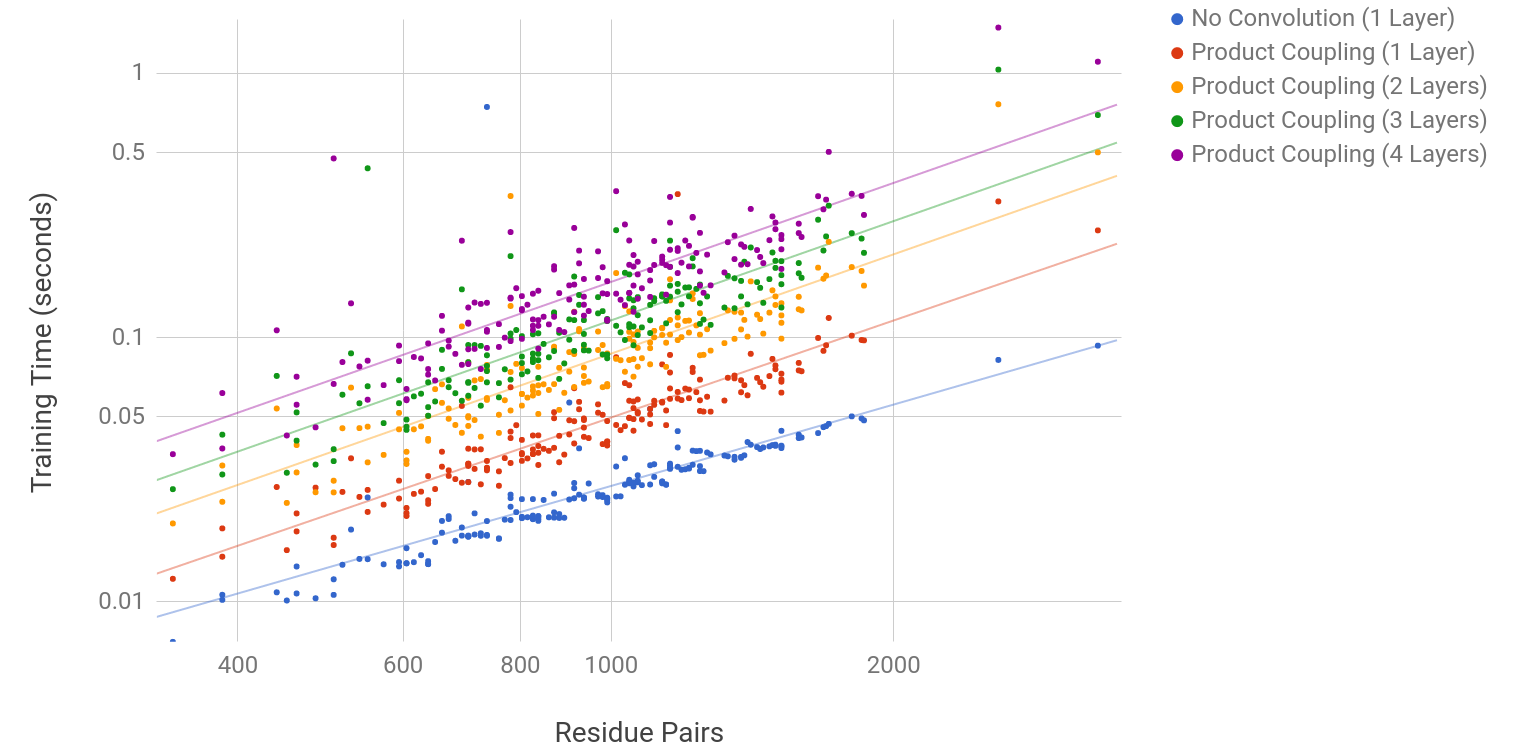
\includegraphics[width=1.0\textwidth]{training_time_product_coupling_1-4.png}
	\caption{Training time as a function of number of residue pairs, for a single No Convolution layer, as well as four depths of Product Coupling, receptive field size 21. Linearity in this log-log plot indicates a power law relationship. In this case, the relationship is near linear, with powers of 1.02, 1.22, 1.25, 1.25, and 1.24 respectively for No Convolution 1 layer, and Product Coupling for 1, 2, 3, and 4 layers. Other convolution methods have similar power law relationships. 
		\label{fig:train_times}}
\end{figure}
